% coding:utf-8

%TV-B-Gone
%Copyright (C) 2013, Daniel Winz, Ervin Mazlagic

%This program is free software; you can redistribute it and/or
%modify it under the terms of the GNU General Public License
%as published by the Free Software Foundation; either version 2
%of the License, or (at your option) any later version.

%This program is distributed in the hope that it will be useful,
%but WITHOUT ANY WARRANTY; without even the implied warranty of
%MERCHANTABILITY or FITNESS FOR A PARTICULAR PURPOSE.  See the
%GNU General Public License for more details.
%----------------------------------------

\section{RC5}
Im Folgenden sollen alle wichtigen Facts zu und über RC5 gegeben werden.

\subsection{Protokoll}
Hier die wichtigsten Facts 
\begin{itemize}
    \item Codelänge beträgt 24.889ms
    \item Pause zwischen Wiederholungen beträgt 88.889ms
    \item Code ist \emph{biphase}-coded\footnote{
        \emph{biphase-coded} kann frei als Flankengetriggert übersetzt
        werden. Siehe Codebeispiel im Bild \ref{pic:rc5_simple} }
    \item Code besteht aus 14-Bit Word
    \begin{itemize}
        \item 2 Start Bits
        \item 1 Toggle Bit
        \item 5 Systemadress-Bits
        \item 6 Kommando-Bits
    \end{itemize}
\end{itemize}

\begin{figure}[h!]
    \centering
    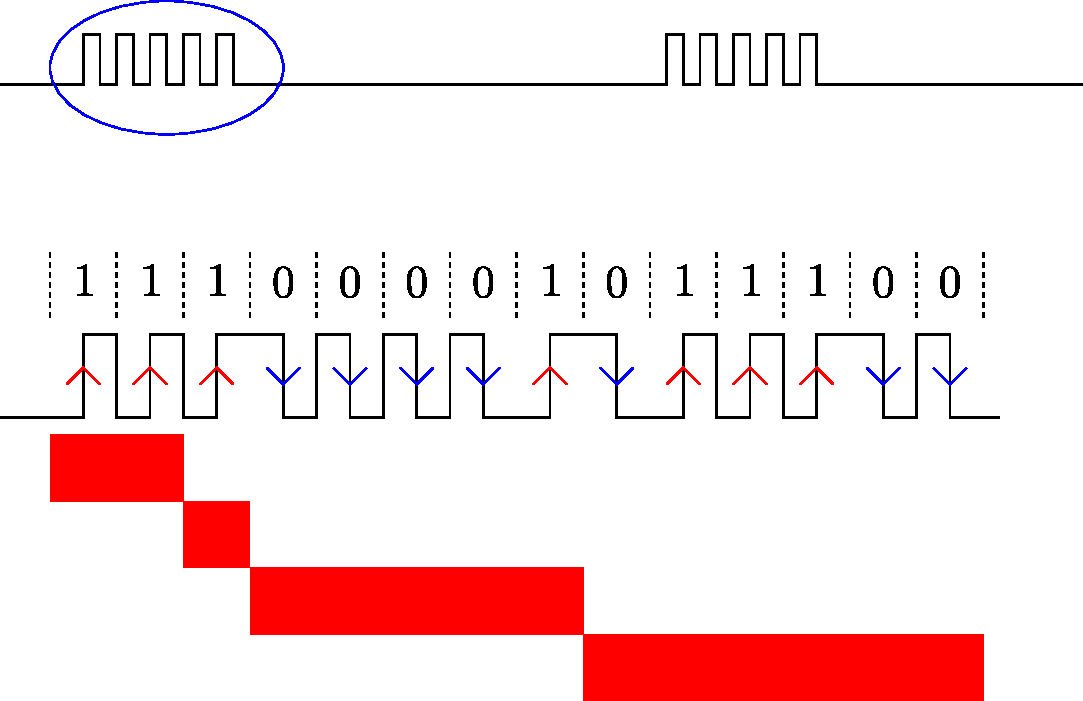
\includegraphics[width=0.8\textwidth]{rc5_simple.pdf}
    \label{pic:rc5_simple}
    \caption{RC5 Protokoll}
\end{figure}

\subsubsection{Start-Bits}
Das Startsignal besteht aus zwei Bits. Zuerst das eigentliche Start-Bit
und dann das sogenannte Field-Bit. Das Startbit ist immer logisch 1 und
stellt beim Empfänger die Verstärkung ein zum einlesen der Daten.
Das Field-Bit wird verwendet um dem Empfänger mitzuteilen, ob man den
unteren (0-63) oder oberen (64-127) Kommandobereich verwendet.

\subsubsection{Toggle-Bit}
Das Toggle- oder auch Steuer-Bit wird dazu verwendet permanentes (bzw. 
wiederholendes) senden von neuem Senden zu unterscheiden.
Dies ist nützlich um z.b. zu erkennen ob eine Taste dauerhaft gedrückt ist
bei der Fernbedienung etc.

\subsubsection{Systemadress-Bits}
Die 5 Systemadress-Bits erlauben es zwischen 32 verschiedenen Geräten
zu operieren.

\subsubsection{Kommando-Bits}
Die 6 Kommando-Bits bieten ein Set von 64 Befehlen an, mit welchem ein
Gerät (welches mit den 5 Systemadress-Bits spezifiziert wurde) angesteuert
werden kann.

\subsubsection{Modulation}
Die Übertragung der einzelnen Bits erfolgt moduliert. Dabei wird bei aktivem
Signal eine Pulsfolge übertragen. Die Pulsdauer beträgt dabei 6.944$\mu$s. 
Dieser Puls wird für jedes Bit 32 mal übertragen. Die Pausenzeit zwischen den Pulsen beträgt 20.833$\mu$s. Dies ergibt eine Periodendauer von 27.777$\mu$s, was einer Frequenz von 36kHz entspricht. 
\begin{figure}[h!]
    \centering
    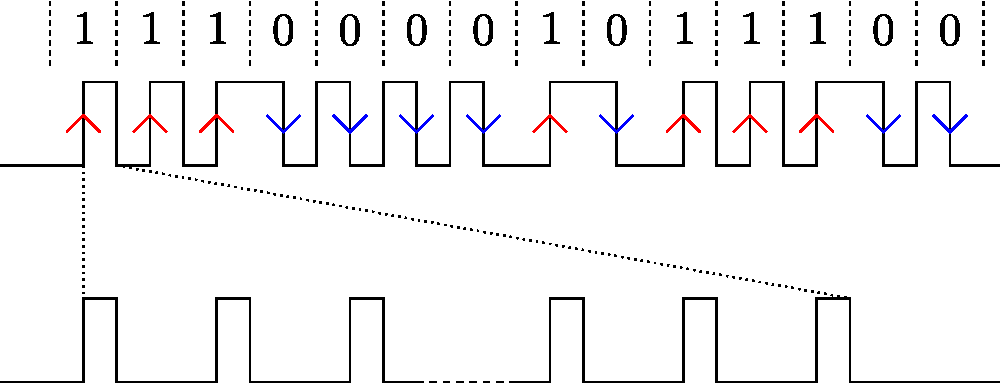
\includegraphics[width=0.8\textwidth]{rc5_modul.pdf}
    \label{pic:rc5_modul}
    \caption{RC5 Modulation}
\end{figure}

\subsection{System-Adressen}

\begin{table}[h!]
    \footnotesize
    \centering
    \begin{tabular}{c l c l c l c l}
    Adresse & Gerät & Adresse & Gerät & Adresse & Gerät & Adresse & Gerät 
    \\
    \hline &&&&&&& \\
    00      & TV1       & 08 & Sat.-Rec 1   & 16 & Audio-PreAmp 1       & 24 & -                \\
    01      & TV2       & 09 & Camera       & 17 & Reciever/Tuner       & 25 & -                \\
    02      & Teletext  & 10 & Sat.-Rec 2   & 18 & Audio Tape Rec.      & 26 & CDR              \\
    03      & Video VD  & 11 & -            & 19 & Audio PreAmp 2$^*$   & 27 & -                \\
    04      & Video LV1 & 12 & Video-CD     & 20 & CD-Player            & 28 & -                \\
    05      & VCR1      & 13 & Camcorder    & 21 & Plattenspieler       & 29 & Beleuchtung 1    \\
    06      & VCR2      & 14 & -            & 22 & -                    & 30 & Beleuchtung 2    \\
    07      & exp.      & 15 & -            & 23 & DAT-T./MD-Rec.       & 31 & Telefon          \\
    \end{tabular}
    \caption{RC5 Systemadressen}
    \label{tab:rc5_systemadressen}
\end{table}
